\subsection{Performance}

\begin{frame}{Measuring time}
    \begin{block}{}
        Performance evaluation metric: amount of clock cycles
        \begin{itemize}
            \item \texttt{DWT\_CYCCNT} register for Cortex-M4
            \item \texttt{rtdsc} instruction for x86
        \end{itemize}
        Measurements are averaged over 1000 runs.\\
        Repeat measurements while varying the amount of memory wait states.
        \begin{itemize}
            \item 16, 32, 48, 64 and 80 MHz on ARM
            \item 2GHz + no TurboBoost on x86
        \end{itemize}
    \end{block}
\end{frame}

\begin{frame}{Timing results}
    \newcommand{\ARMtimingplot}[1]{
    \begin{tikzpicture}
        \centering
        \begin{axis}[
            height=70mm, width=150mm,
        %
            bar width=0.1,
            ybar=2pt,
            enlarge x limits={abs=0.5},
            %ymin=0,
            %ymax=170000,
            %ytick distance=10000,
            yticklabel style={font=\small},
            yticklabel=\pgfmathprintnumber{\tick},
            ylabel={Execution time (kcycles)},
            xlabel={Wait States},
            xtick=data,
            xticklabels from table={#1}{Label},
        %
            %nodes near coords,
            %nodes near coords style={font=\tiny,
            %                        /pgf/number format/.cd,
            %                                    precision=0,
            %                                    zerofill,
            %                        },
            legend style={legend pos=north east,
                        cells={anchor=west},
                        font=\footnotesize,
                        }
        ]
        \addplot table [x expr=\coordindex,y=Reference (R3)]{#1};
        \addplot table [x expr=\coordindex,y=sparsemul (R3)]{#1};
        %\addplot table [x expr=\coordindex,y=Reference (R4)]{#1};
        \addplot table [x expr=\coordindex,y=sparsemul (R4)]{#1};
        \addplot table [x expr=\coordindex,y=FAFFT (R4)]{#1};
        \legend{Reference (R3), sparsemul (R3), sparsemul (R4), FAFFT (R4)}    
        \end{axis}
    \end{tikzpicture}
}
    \pgfplotstableread[col sep=comma]{  % enc
    Label, Reference (R3), sparsemul (R3), Reference (R4), sparsemul (R4), FAFFT (R4)
    0,      2726,          18920,           136262,         18965,          8834
    1,      2748,          18937,           138227,         18991,          10107
    2,      2799,          18986,           142093,         19049,          11595
    3,      2886,          19064,           147971,         19154,          13189
    4,      3035,          19196,           155762,         19324,          14856
}\armEncTiming % enc

\pgfplotstableread[col sep=comma]{  % dec
    Label,               Reference (R3), sparsemul (R3), Reference (R4), sparsemul (R3), FAFFT (R4)
    0,                 1942,           9010,           68750,          8915,           5043
    1,                 1950,           9018,           69733,          8926,           5677
    2,                 1965,           9027,           71657,          8941,           6409
    3,                 1989,           9045,           74568,          8958,           7176
    4,                 2024,           9071,           78415,          8998,           7958
}\armDecTiming

\pgfplotstableread[col sep=comma]{  % encaps
    Label,           Reference (R3), sparsemul (R3), Reference (R4), sparsemul (R4), FAFFT (R4)
    0,                 3913,           20105,          137873,         20571,          10441
    1,                 3958,           20148,          139835,         20643,          11763
    2,                 4079,           20261,          143631,         20783,          13333
    3,                 4289,           20461,          149685,         21051,          15087
    4,                 4626,           20787,          157722,         21473,          16994
}\armEncapsTiming

\pgfplotstableread[col sep=comma]{  % decaps
    Label,               Reference (R3), sparsemul (R3), Reference (R4), sparsemul (R4), FAFFT (R4)
    0,                 5923,           29182,          206691,         29557,          15546
    1,                 5974,           29230,          209618,         29634,          17504
    2,                 6110,           29361,          215263,         29795,          19804
    3,                 6341,           29578,          224238,         30084,          22326
    4,                 6724,           29926,          236118,         30540,          25015
}\armDecapsTiming

\pgfplotstableread[col sep=comma]{  % mult
    Label,               Reference (R3), sparsemul (R3), Reference (R4), sparsemul (R4), FAFFT (R4)
    0,                 848,            7897,           66777,          7791,           3062
    1,                 848,            7897,           67747,          7791,           3688
    2,                 851,            7897,           69653,          7791,           4404
    3,                 856,            7897,           72537,          7791,           5146
    4,                 862,            7897,           76345,          7791,           5892
}\armMultTiming
  % contains data for the plots
    \pgfplotstableread[col sep=comma]{  % dec
    Label,               Reference (R3), sparsemul (R3), Reference (R4), sparsemul (R4), FAFFT (R4)
    Encrypt,                148,           604,           157,          667,           1212
    Decrypt,                219,           370,           185,          396,           757
    Encaps,                 216,           667,           220,          727,           1278
    Decaps,                 440,           1041,          407,          1145,          2041
}\mydata
  % contains data for the plots

    \begin{figure}
        \centering
        \begin{tikzpicture}
            \centering
            \begin{axis}[
                height=65mm, width=120mm,
                bar width=0.15,
                ybar=0pt,
                enlarge x limits={abs=0.5},
                ymode=log,
                log basis y=10,
                yticklabel style={font=\small},
                xlabel={Wait States},
                ylabel={Execution time (kcycles)},
                xtick=data,
                point meta=rawy,
                grid style={line width=.2pt, draw=gray!20},
                grid=minor,
            ]
            \addplot[preaction={fill=blue!30}, pattern=north west lines, pattern color=blue!50!black] table [x expr=\coordindex, y=reference (R3)]{\armMultTiming};
            \addplot[preaction={fill=red!30}, pattern=crosshatch dots, pattern color=purple!70] table [x expr=\coordindex, y=reference (R4)]{\armMultTiming};
            \addplot[preaction={fill=yellow!30}, pattern=north east lines, pattern color=orange!70] table [x expr=\coordindex, y=sparsemul]{\armMultTiming};
            \addplot[preaction={fill=green!30}, pattern=crosshatch, pattern color=green!40!black] table [x expr=\coordindex, y=fastmul]{\armMultTiming};
            \end{axis}
        \end{tikzpicture}
        \newline
        \begin{tikzpicture}
            \draw[fill=white, draw=black] (-0.5, -0.4) rectangle (11.6, 0.4);
            \node [draw, preaction={fill=blue!30}, pattern=north west lines, pattern color=blue!50!black, rectangle, minimum width=0.3cm, minimum height=0.3cm] (box1) {};
            \node [right=0.01cm of box1] (text1) {\small Shift\&Add};
            \node [draw, preaction={fill=red!30}, pattern=crosshatch, pattern color=purple!70, rectangle, minimum width=0.3cm, minimum height=0.3cm, right=0.5cm of text1] (box2) {};
            \node [right=0.01cm of box2] (text2) {\small Karatsuba$^{\dagger}$};
            \node [draw, preaction={fill=yellow!30}, pattern=north east lines, pattern color=orange!70, rectangle, minimum width=0.3cm, minimum height=0.3cm, right=0.5cm of text2] (box3) {};
            \node [right=0.01cm of box3] (text3) {\small CT Shift\&Add$^{\dagger}$};
            \node [draw, preaction={fill=green!30}, pattern=crosshatch, pattern color=green!40!black, rectangle, minimum width=0.3cm, minimum height=0.3cm, right=0.5cm of text3] (box4) {};
            \node [right=0.01cm of box4] (text4) {\small Frobenius FFT};
        \end{tikzpicture}
    \end{figure}
\end{frame}

\subsection{Side-channel resistance}

\begin{frame}{Test Vector Leakage Assessment}
    \begin{block}{Statistical t-test}
       Determine how much the means of two populations differ by evaluating
       \begin{equation*}
            t = \frac{\mu_0 - \mu_1}{\sqrt{\frac{s_0^2}{n_0} + \frac{s_1^2}{n_1}}}
       \end{equation*}
        A t-value $|t| < 4.5$ implies that the populations have the same mean with 99.999\% confidence. 
    \end{block}
    \begin{block}{}
        Populations to be measured (1000 rounds each)
        \begin{itemize}
            \item fixed inputs 
            \item random inputs 
        \end{itemize}
        Randomness is always generated by the onboard TRNG.
    \end{block}
\end{frame} 

\begin{frame}{Constant-time: multiplication}
    \begin{block}{}
        \begin{table}[H]
    \centering
    \caption{t-values for the multiplication algorithms}
    \begin{tabular}{c|cccc}
        \toprule
        & \textbf{Shift\&Add} & \textbf{Karatsuba} & \textbf{CT Shift\&Add} & \textbf{Frobenius FFT} \\
        \midrule
        \texttt{ARM} & 55.748 & 0.000 & 0.000 & 0.000 \\
        \texttt{x86} & 20.936 & 3.644 & 3.371 & 1.232\\
        \bottomrule
    \end{tabular}
    \label{tab:ctmult}
\end{table}
    \end{block}
    \begin{block}{}
        All algorithms except plain S\&A are constant-time, we choose
        \begin{itemize}
            \item Frobenius FFT on ARM
            \item Karatsuba (with AVX) on x86
        \end{itemize}
    \end{block}
\end{frame}

\begin{frame}{Constant-time: PKE}
    \begin{block}{}
        \begin{table}[H]\footnotesize
            \centering
            \begin{tabular}{c | c c c | c c | c c}
                \toprule
                & & & &  \multicolumn{2}{c|}{\textbf{Encrypt}} & \multicolumn{2}{c}{\textbf{Decrypt}}\\
                \textbf{Round} & \textbf{Version} & \textbf{Mul} & \textbf{CT?} & \texttt{x86} & \texttt{ARM} & \texttt{x86} & \texttt{ARM} \\
                \midrule
                \multirow{2}{*}{3}
                & \tt{reference} & Shift\&Add & $\circ$ & 10.65 & 29.19 & 5.59 & 39.23 \\
                & \tt{sparsemul} & CT Shift\&Add$^\dagger$ & $\bullet$ & 9.38 & 23.12 & 7.59 & 49.56 \\
                \midrule
                \multirow{3}{*}{4}
                & \tt{reference} & Karatsuba$^\dagger$ & $\bullet$ & 1.27 & 1.04 & 0.97 & 0.30 \\
                & \tt{sparsemul} & CT Shift\&Add$^\dagger$ & $\bullet$ & 0.29 & 0.07 & 1.51 & 1.64 \\
                & \tt{fastmul} & Frobenius FFT & $\bullet$ & 3.36 & 0.56 & 1.70 & 1.99 \\
                \bottomrule
            \end{tabular}
        \end{table}
    \end{block}
\end{frame}

\begin{frame}{Constant-time: KEM}
    \begin{block}{}
        \begin{table}[H]\footnotesize
            \centering
            \begin{tabular}{c | c c c | c c | c c}
                \toprule
                & & & &  \multicolumn{2}{c|}{\textbf{Encaps}} & \multicolumn{2}{c}{\textbf{Decaps}}\\
                \textbf{Round} & \textbf{Version} & \textbf{Mul} & \textbf{CT?} & \texttt{x86} & \texttt{ARM} & \texttt{x86} & \texttt{ARM} \\
                \midrule
                \multirow{2}{*}{3}
                & \tt{reference} & Shift\&Add & $\circ$ & 58.42 & 28.65 & 20.71 & 18.44\\
                & \tt{sparsemul} & CT Shift\&Add$^\dagger$ & $\bullet$ & 6.75 & 14.29 & 5.81 & 23.70 \\
                \midrule
                \multirow{3}{*}{4}
                & \tt{reference} & Karatsuba$^\dagger$ & $\bullet$ & 3.77 & 4.01 & 4.56 & 0.26\\
                & \tt{sparsemul} & CT Shift\&Add$^\dagger$ & $\bullet$ & 1.58 & 2.17 & 1.04 & 0.22 \\
                & \tt{fastmul} & Frobenius FFT & $\bullet$ & 4.31 & 4.25 & 2.41 & 0.53 \\
                \bottomrule
            \end{tabular}
        \end{table}
    \end{block}
\end{frame}

\begin{frame}{Power measurements}
    \begin{block}{Setup}
        Measure the EM radiation emitted by the board package (non invasive)
    \end{block}
    \begin{figure}
        \centering
        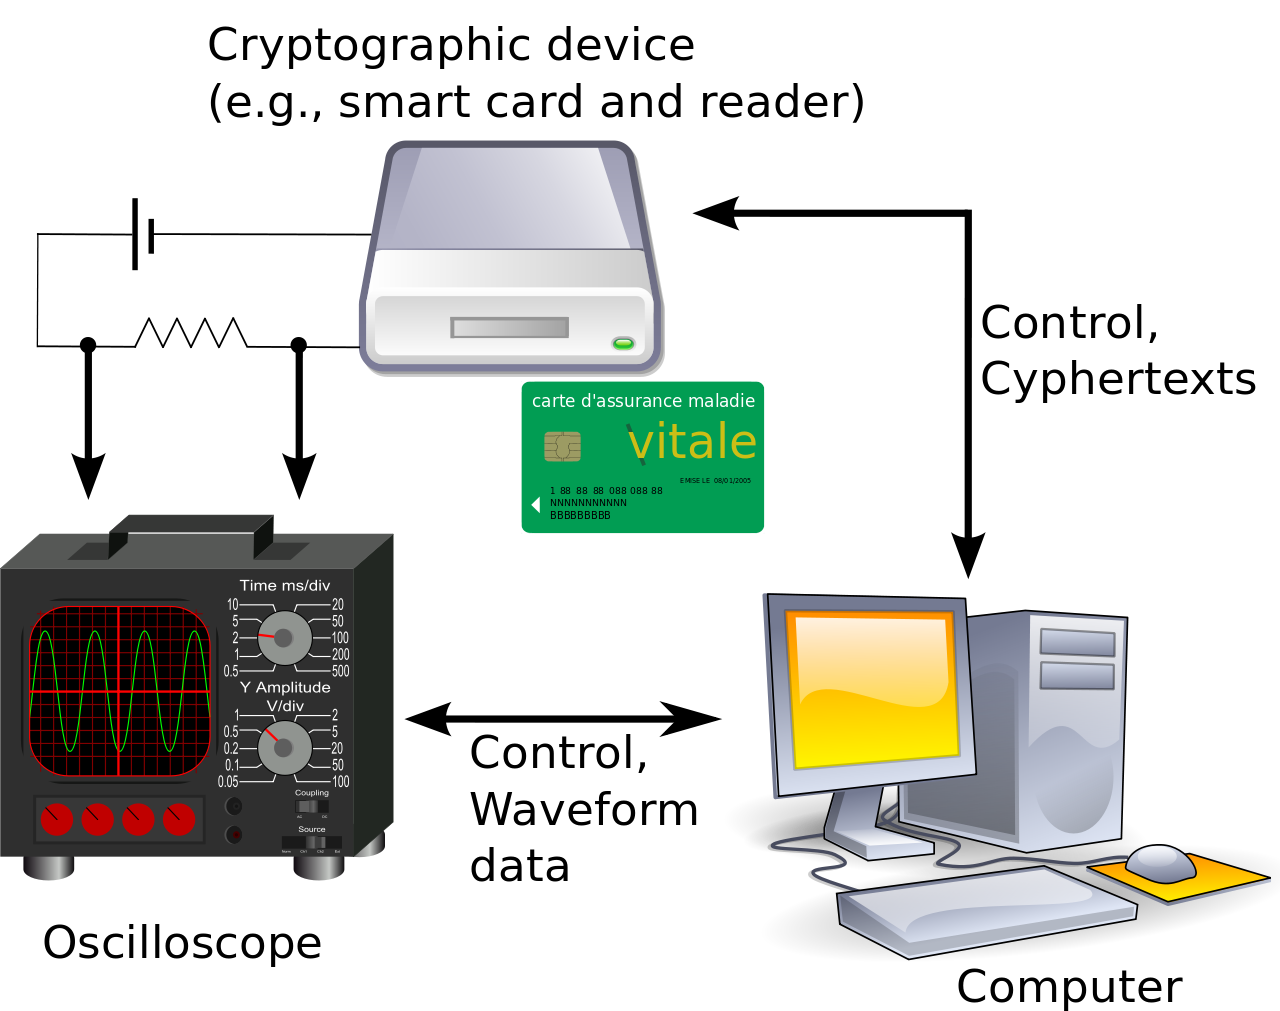
\includegraphics[scale=0.15]{beamer/images/power.png}
    \end{figure}
\end{frame}

\begin{frame}{EM t-values: decoder}
    \begin{figure}
        \centering
        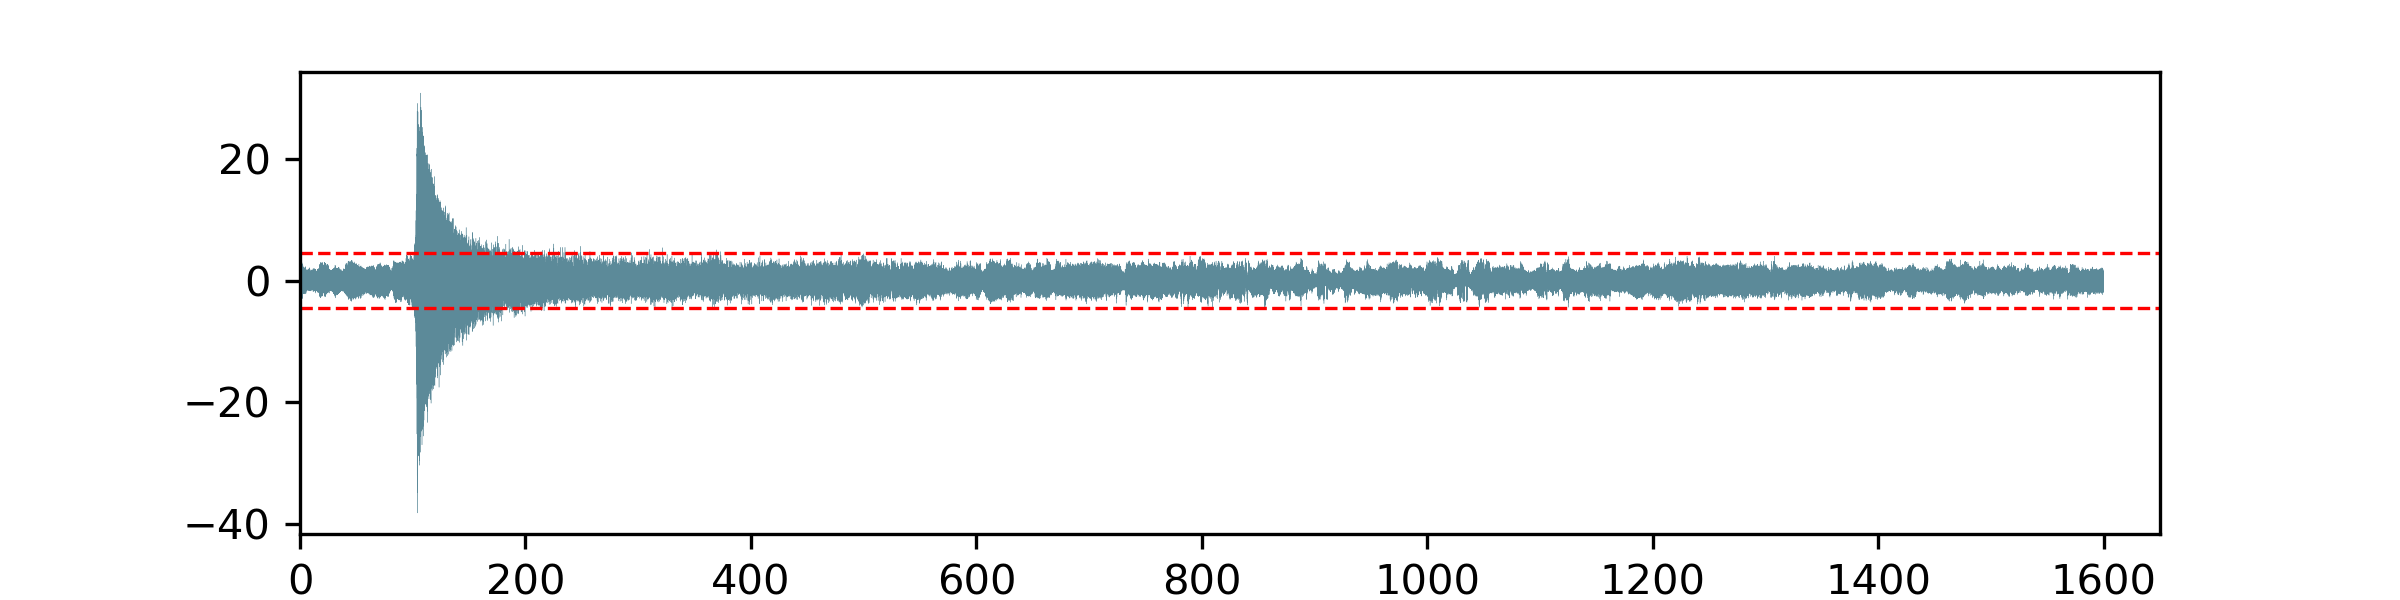
\includegraphics[scale=0.65]{beamer/images/rsdecode_nomask.png}
        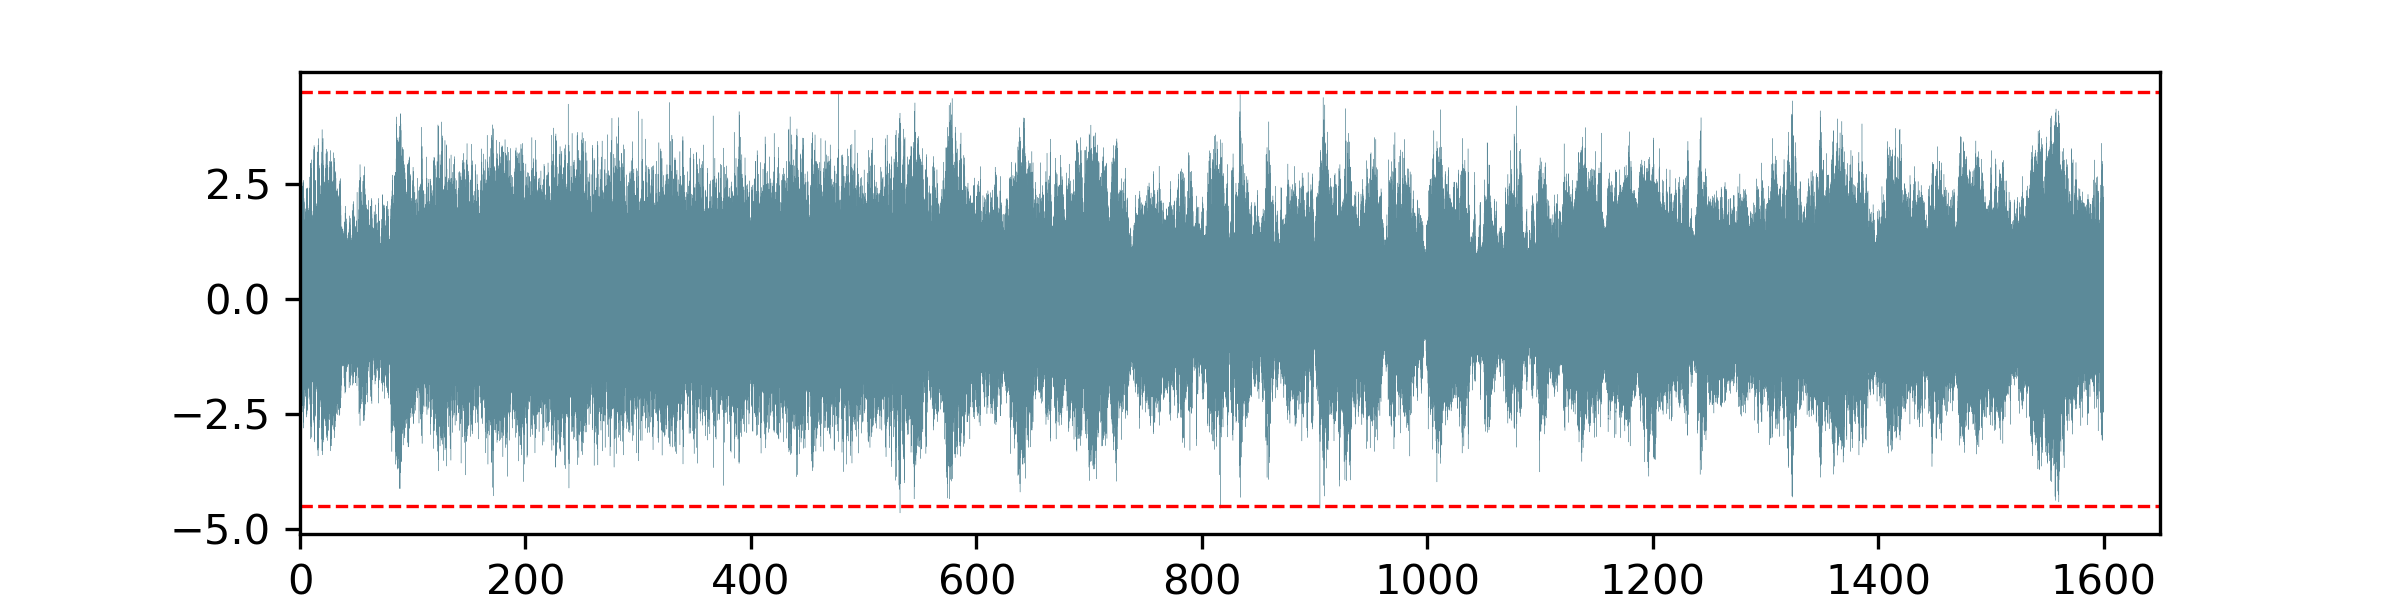
\includegraphics[scale=0.65]{beamer/images/rsdecode_masked.png}
    \end{figure}
\end{frame}

\subsection{Comparison with other cryptosystems}

\begin{frame}{Execution time}
    \begin{figure}[H]
        \centering
        \pgfplotstableread[col sep=comma, row sep=crcr]{ % data 
            Label, Keygen, Encaps, Decaps\\
            McEliece, 2146932, 582, 2706\\
            BIKE, 24935, 3253, 49911\\
            HQC, 4934, 10441, 15546\\
            HQC(masked), 8228, 17050, 25522\\
        }\mydata
        \begin{tikzpicture}
        \centering
        \begin{axis}[
            height=60mm, width=120mm,
    %
            bar width=0.22,
            ybar=0pt,
            enlarge x limits={abs=0.5},
            ymin=0,
            ymax=55000,
            ytick distance=10000,
            yticklabel style={font=\small},
            yticklabel=\pgfmathprintnumber{\tick},
            ylabel={Execution time (kcycles)},
            %xlabel={Cryptosystem},
            xtick=data,
            xticklabels from table={\mydata}{Label},
            grid style={line width=.2pt, draw=gray!20},            
            ymajorgrids=true,
    %
            nodes near coords,
            nodes near coords style={font=\tiny,
                                    /pgf/number format/.cd,
                                                precision=0,
                                                zerofill,
                                    },
        ]
    \addplot[preaction={fill=blue!30}, pattern=north west lines, pattern color=blue!50!black] table [x expr=\coordindex,y=Keygen]{\mydata};
    \addplot[preaction={fill=red!30}, pattern=crosshatch dots, pattern color=purple!70] table [x expr=\coordindex,y=Encaps]{\mydata};
    \addplot[preaction={fill=yellow!30}, pattern=north east lines, pattern color=orange!70] table [x expr=\coordindex,y=Decaps]{\mydata};
    \end{axis}
    \end{tikzpicture}
    
    \begin{tikzpicture}
        % draw a rectangle around all
        \draw[fill=white, draw=black] (-0.5, -0.4) rectangle (8, 0.4);
        \node [draw, preaction={fill=blue!30}, pattern=north west lines, pattern color=blue!50!black, rectangle, minimum width=0.3cm, minimum height=0.3cm] (box1) {};
        \node [right=0.01cm of box1] (text1) {\small Keygen};
        \node [draw, preaction={fill=red!30}, pattern=crosshatch dots, pattern color=purple!70, rectangle, minimum width=0.3cm, minimum height=0.3cm, right=0.5cm of text1] (box2) {};
        \node [right=0.01cm of box2] (text2) {\small Encapsulation};
        \node [draw, preaction={fill=yellow!30}, pattern=north east lines, pattern color=orange!70, rectangle, minimum width=0.3cm, minimum height=0.3cm, right=0.5cm of text2] (box3) {};
        \node [right=0.01cm of box3] (text3) {\small Decapsulation};
    \end{tikzpicture}
    \end{figure}
\end{frame}

\begin{frame}{Memory}
    \begin{figure}[H]
        \centering
    \pgfplotstableread[col sep=comma, row sep=crcr]{ % data 
    Label,     pk, sk, ctx\\
    McEliece, 261120, 6492, 128\\
    BIKE, 1540, 280, 1572\\
    HQC, 2249, 40, 4481\\
        }\memorytable
        \begin{tikzpicture}
        \centering
        \begin{axis}[
            height=60mm, width=119mm,
    %
            bar width=0.22,
            ybar=0pt,
            enlarge x limits={abs=0.5},
            ymin=0,
            ymax=8000,
            ytick distance=1000,
            yticklabel style={font=\small},
            yticklabel=\pgfmathprintnumber{\tick},
            ylabel={Memory usage (Bytes)},
            %xlabel={Cryptosystem},
            xtick=data,
            xticklabels from table={\memorytable}{Label},
            grid style={line width=.2pt, draw=gray!20},            
            ymajorgrids=true,
    %
            nodes near coords,
            nodes near coords style={font=\tiny,
                                    /pgf/number format/.cd,
                                                precision=0,
                                                zerofill,
                                    },
            legend style={legend pos=north east,
                        cells={anchor=west},
                        font=\footnotesize,
                        }
        ]
    \addplot[preaction={fill=blue!30}, pattern=north west lines, pattern color=blue!50!black] table [x expr=\coordindex,y=pk]{\memorytable};
    \addplot[preaction={fill=red!30}, pattern=crosshatch dots, pattern color=purple!70] table [x expr=\coordindex,y=sk]{\memorytable};
    \addplot[preaction={fill=yellow!30}, pattern=north east lines, pattern color=orange!70] table [x expr=\coordindex,y=ctx]{\memorytable};
    \end{axis}
        \end{tikzpicture}
    
        \begin{tikzpicture}
            % draw a rectangle around all
            \draw[fill=white, draw=black] (-0.5, -0.4) rectangle (7.5, 0.4);
            \node [draw, preaction={fill=blue!30}, pattern=north west lines, pattern color=blue!50!black, rectangle, minimum width=0.3cm, minimum height=0.3cm] (box1) {};
            \node [right=0.01cm of box1] (text1) {\small Public key};
            \node [draw, preaction={fill=red!30}, pattern=crosshatch dots, pattern color=purple!70, rectangle, minimum width=0.3cm, minimum height=0.3cm, right=0.5cm of text1] (box2) {};
            \node [right=0.01cm of box2] (text2) {\small Secret Key};
            \node [draw, preaction={fill=yellow!30}, pattern=north east lines, pattern color=orange!70, rectangle, minimum width=0.3cm, minimum height=0.3cm, right=0.5cm of text2] (box3) {};
            \node [right=0.01cm of box3] (text3) {\small Ciphertext};
        \end{tikzpicture}
    \end{figure}
\end{frame}
